\documentclass[a4paper,
               %boxit,
               %titlepage,   % separate title page
               %refpage      % separate references
              ]{jacow}

\ifboolexpr{bool{xetex} or bool{luatex}} % test for XeTeX/LuaTeX
 {}                                      % input encoding is utf8 by default
 {\usepackage[utf8]{inputenc}}           % switch to utf8

\usepackage{graphicx, subfigure}
\usepackage{booktabs}


\begin{document}
\title{BEAM COUPLING IMPEDANCE OF THE NEW BEAM SCREEN OF THE LHC INJECTION KICKER MAGNETS}
\author{H. Day\thanks{hugo.day@hep.manchester.ac.uk}$^{\dagger}$, M.J. Barnes$^{\dagger}$, F. Caspers$^{\dagger}$, E. Métral$^{\dagger}$, B. Salvant$^{\dagger}$, J. Uythoven$^{\dagger}$ \\
$\dagger$ CERN, Switzerland
}

\maketitle 


\begin{abstract}
The LHC injection kicker magnets experienced significant beam induced heating of the ferrite yoke, with high intensity beam circulating for many hours, during operation of the LHC in 2011 and 2012. The causes of this beam coupling impedance were studied in depth and an improved beam screen implemented to reduce the impedance. Results of measurements and simulations of the new beam screen design are presented in this paper: these are used to predict power loss and temperature of the ferrite yoke for operation after long shutdown 1 and for proposed HL-LHC operational parameters.
\end{abstract}

\section{Introduction}

During the 2011 and 2012 runs of the LHC, high temperatures were observed in several devices in the LHC  \cite{metral_cham2012}, a critical piece being the LHC injection kicker magnets (MKIs) Fig.~\ref{fig:mkiStruct}, which were attributed to beam-induced heating due to high power loss from the interaction of the circulating beam with the longitudinal beam coupling impedance. This heating was observed to raise the temperature of the ferrite yoke of one of the MKIs above its Curie point during fills, thereby necessitating waiting times of several hours for the ferrite to cool before safe injection could be carried out \cite{mki-heating}. The MKIs are fast pulsed transmission line kicker magnets, which has a ceramic beam screen inserted into the ferrite yoke which supports a number of screen conductors designed to provide a good conducting path for the image currents of the circulating beam. One end is directly connected to the beam pipe whilst the other is capactively coupled to the beam pipe in order to preserve the fast field rise time of the magnet. Initial design forsaw placing 24 equally spaced screen conductors in the beam screen, however poor HV performance necessitated that the 9 closest to the HV busbar be removed, leaving a large section of the ferrite yoke unscreened. A magnet with an improved beam screen was inserted during technical stop 3 (TS3) (23/09/12-27/09/12), replacing the MKI8D which was measured to have the highest temperature \cite{mki-heatingTemp}; the replacement magnet was subsequently measured to have the lowest temperature of all magnets.

Building on this success a new design has been proposed to satisfy competing needs of low rates of electrical breakdown during magnet pulsing and a low beam coupling impedance to reduce the power lost into the structure by wakefields; in addition to meeting strict requirements for magnet operation for field rise time and flat top stability \cite{mkiUpgrade}. 

\begin{figure}
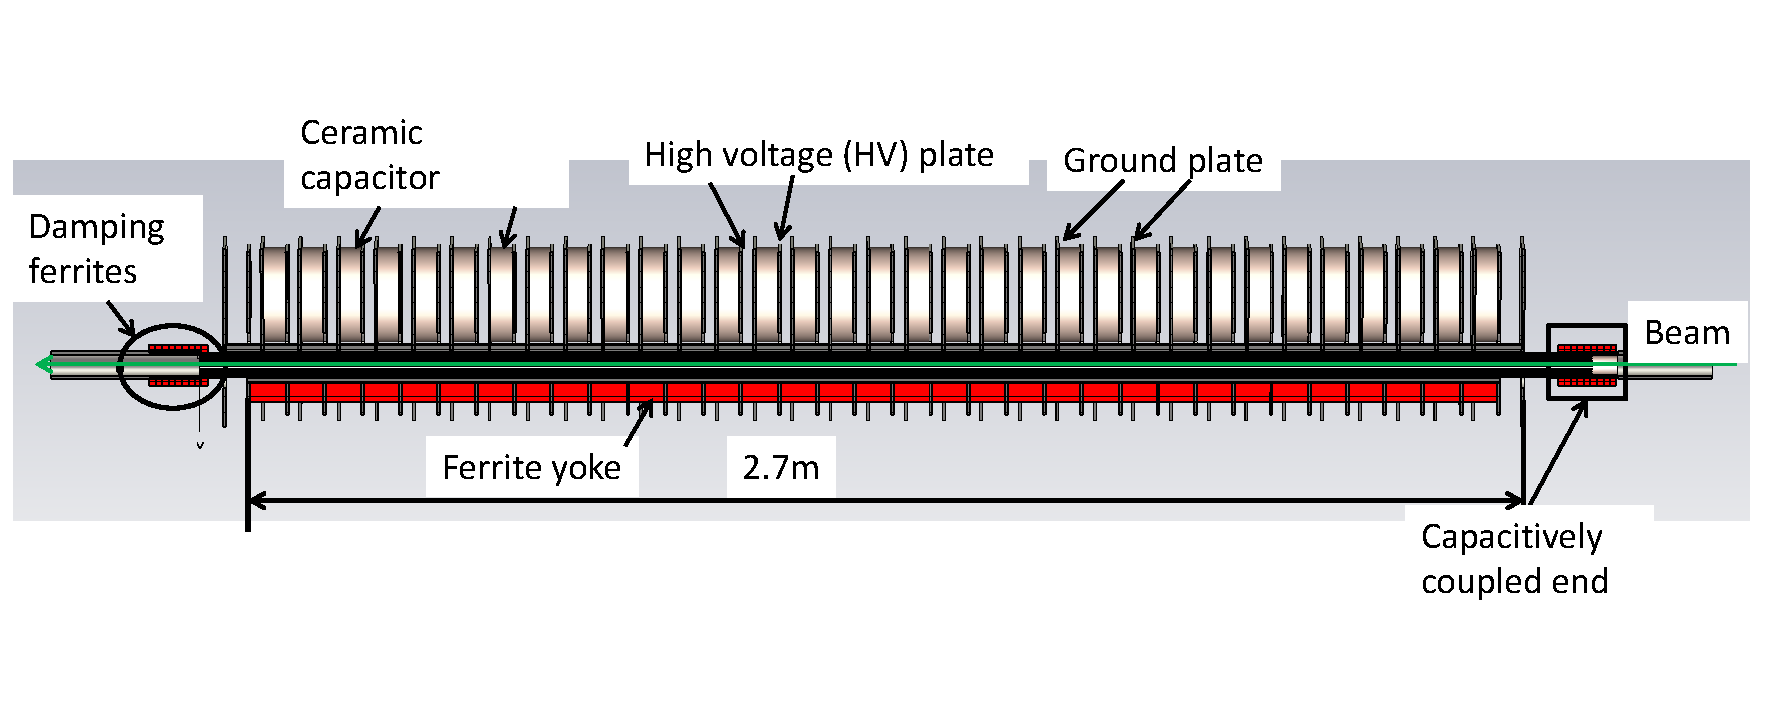
\includegraphics[width=0.5\textwidth]{MKICrossSectionYZ.pdf}
\caption{Structure of the injection kicker magnets.}
\label{fig:mkiStruct}
\end{figure}

\section{New Beam Screen Design}

The new design involves a redesign of the capacitively coupled end of the beam screen, intended to reduce the electrical field due to the induced potentials on the screen conductors during magnet pulsing. This reduced electric field reduces the possibility of surface breakdown on the internal face of the beam screen allowing additional beam screens to be inserted where previously they had been removed due to being located in regions of high electric field Fig.~\ref{fig:beamScreenCross} providing complete screening of the ferrite yoke of the magnet. See \cite{mki-ElecBreakdown} for more information on behaviour relating to surface flashover. 

\begin{figure}
\begin{center}
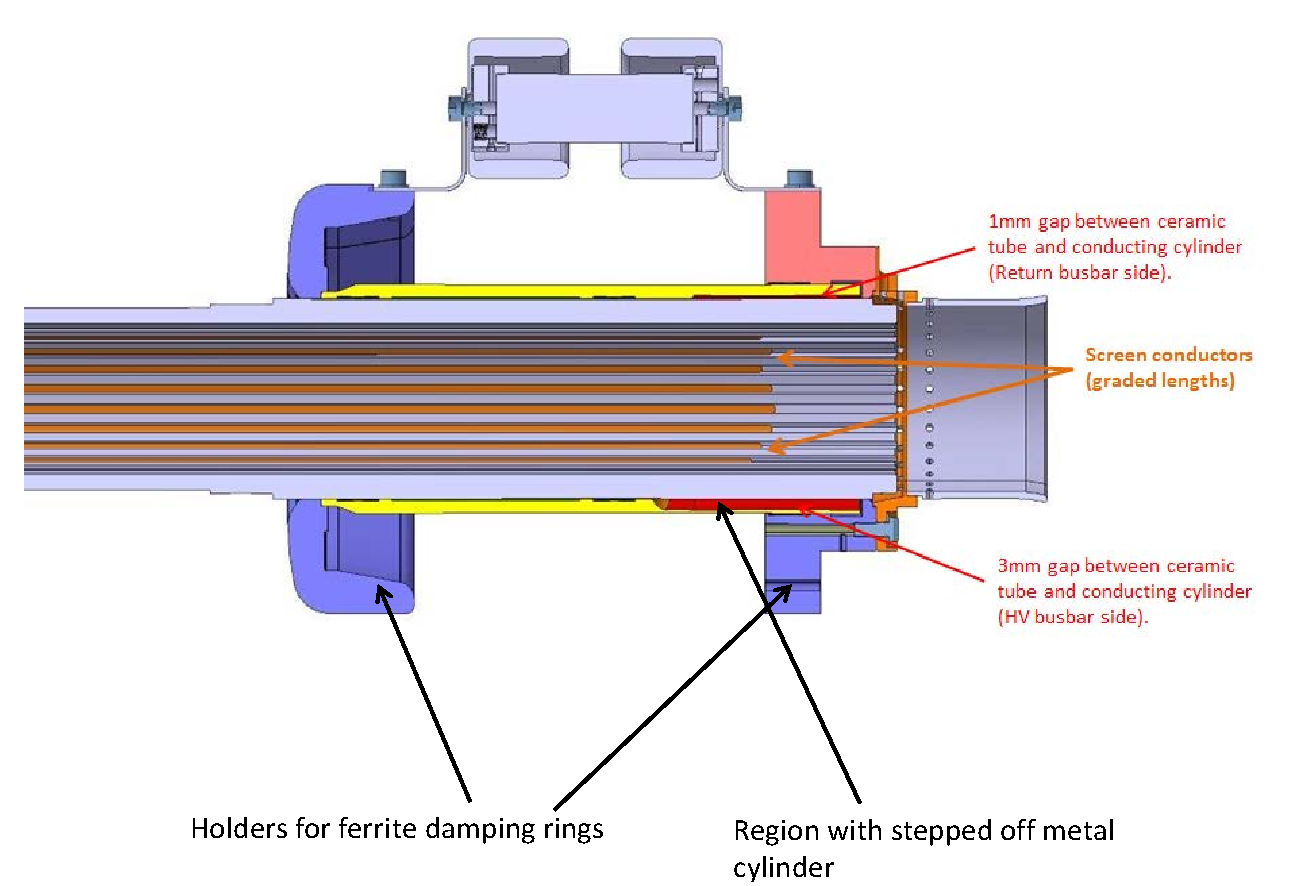
\includegraphics[width=0.45\textwidth]{beamScreenCrossSectionLabelled.pdf}
\caption{Cross section of the new beam screen design}
\label{fig:beamScreenCross}
\end{center}
\end{figure}



\section{Impedance Measurements}

In order to observe the effect of manufacutring tolerences between magnets and as part of the campaign to characterise the impedance of all devices placed into the LHC each of the MKIs with the new beam screen has it's longitudinal beam coupling impedance measured during assembly. These measurements are carried out using the resonant coaxial wire method [cite], a measurement technique that turns the device under test (DUT) into a coaxial resonator with a weak external coupling. This allows very sensitive measurements of the impedance of the DUT to be made, at the cost of a relatively poor frequency resolution as the measurement is of the Q-factor at the resonant frequencies of the coaxial device.

The real component of the longitudinal beam coupling impedance of an example of the new design as well as for an MKI before LS1 (with 15 screen conductors) and the MKI8D that was replaced in TS3 (with 19 screen conductors) are shown in Fig.~\ref{fig:Imp241915}. It can be seen that the new design has a substantially lower beam coupling impedance over the majority of the frequency range, with the broadband impedance seen in the case of 15 screen conductors becoming resonant in nature with 24 conductors. This is due to the improved screening of the ferrite yoke by having 24 screen conductors equally distributed around the beam screen as opposed to an arc of some 135$^{\circ}$ left unscreened when only 15 screen conductors are in place.

\begin{figure}
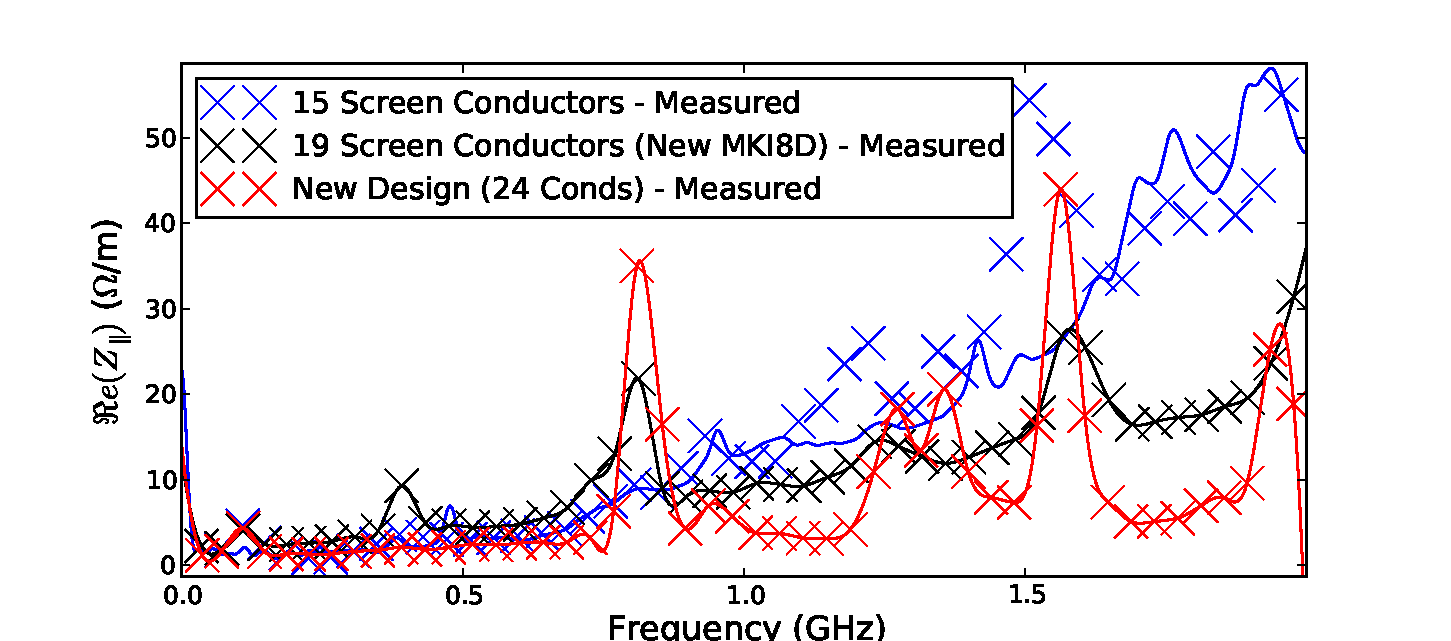
\includegraphics[width=0.5\textwidth]{measImp151924.pdf}
\caption{Real component of the longituidinal beam coupling impedance measured using the resonant coaxial wire method for the new beam screen design, the design with 15 screen conductors as was the case for most magnets prior to LS1 and the upgraded MKI8D, inserted in TS3.}
\label{fig:Imp241915}
\end{figure}

The real component of the longitudinal beam coupling impedance of the 9 MKIs upgraded with the new beam screen design to date (June 2014), measured using the resonant coaxial wire technique. It can be seen that the consistency between the magnets is very good - resonant frequencies are *Res freq +/- error*, with peak impedances of *peak +/- error* for the first measured resonance at 890MHz. This indicates that with the rigorous assembly procedure has eliminated some of the variation in the beam impedance of the MKIs prior to LS1.

\begin{figure}
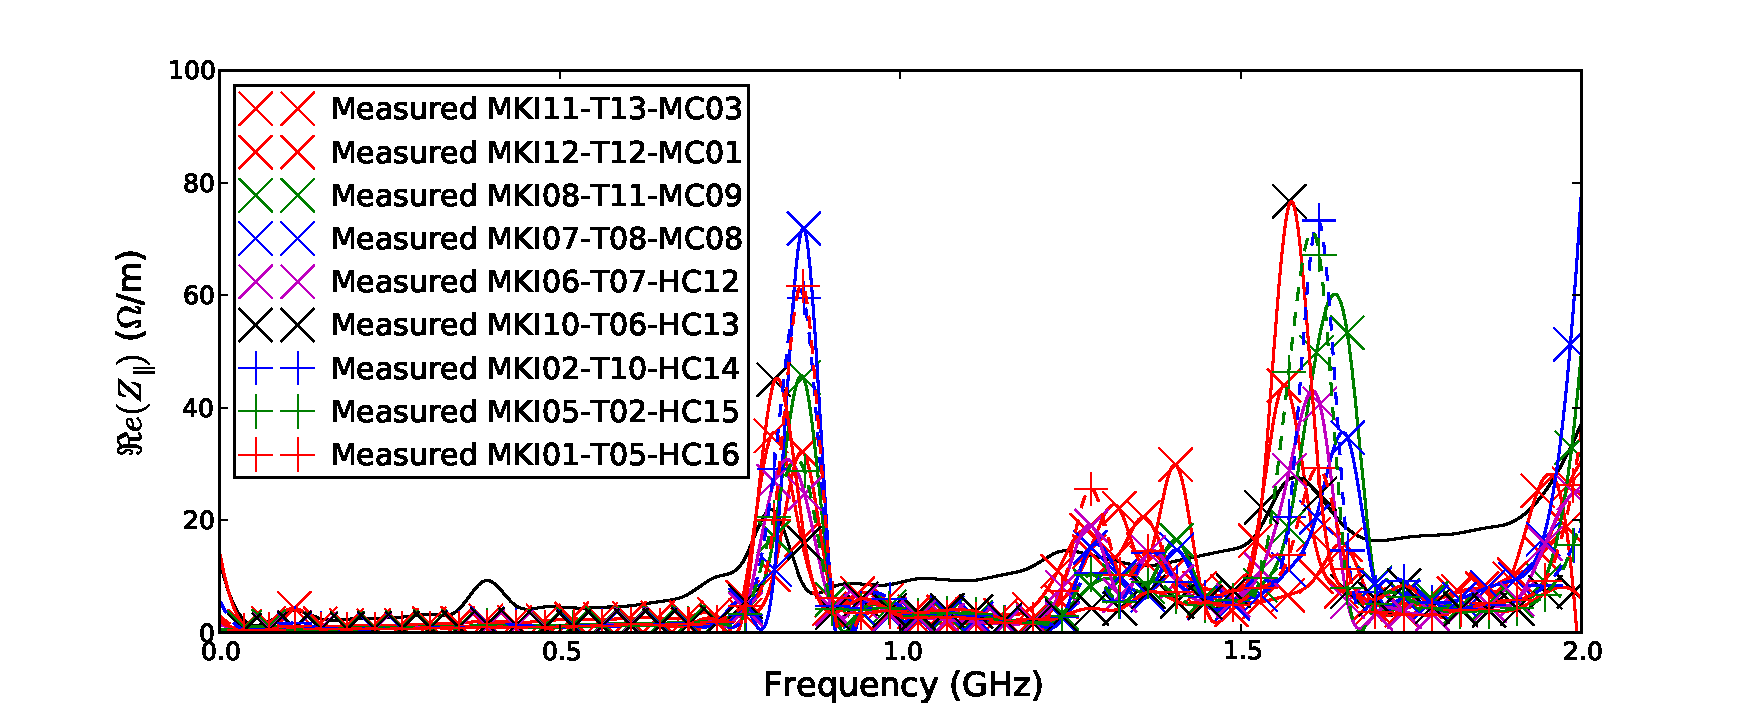
\includegraphics[width=0.5\textwidth]{mkiNewDesignAll.pdf}
\caption{Real component of the longitudinal beam coupling impedance measured using the resonant coaxial wire method for the first 9 magnets fitted with the new beam screen design. 8 are to be installed for use after LS1, with an additional 4 as spares.}
\label{fig:allNewMKIImp}
\end{figure}

To verify the simulations carried out in the design phase of the new design we compare a number of measurement methods. The resonant coaxial wire method provides very good accuracy for the measurements but relatively poor frequency resolution if only the DUT is used in the coaxial resonator; frequency data points are spaced such that $\Delta f \approx \frac{nc}{2L_{DUT}}$, where $n$ is an integer. $c$ the speed of light, $L_{DUT}$ the length of the device measured. The classical coaxial wire technique gives a frequency range determined only by the frequency points on the network analyser, however any residual mismatch in the characteristic impedance between the measurement network and the DUT will result in reflections in the system which limits the achieveable accuracy. Alternatively it's possible to use time domain gating to gate out reflected signals, however due to the varying characteristic impedance along the length of the DUT it's difficult to gate all reflections without losing sensitivity in the measurements.

A comparison of the beam coupling impedance for each signal is shown in Fig.~\ref{fig:measComp}. The frequency domain data for the time domain gated measurement is processed to give a beam coupling impedance it can be seen that there is a large DC offset, caused by the loss of transmitted energy by the gating of the signal. The resistively matched measurements give good results below $\approx$ 500 MHz but the residual mismatch in the system (characteristic impedance of DUT $Z_{c}^{DUT}\approx 270$ was matched used a carbon film resistor of 220 $\Omega$) causes large oscillations which mask the true impedance. It can be seen that although the gated and matched network measurements give useful information, particularly the presence of not of  

\begin{figure}
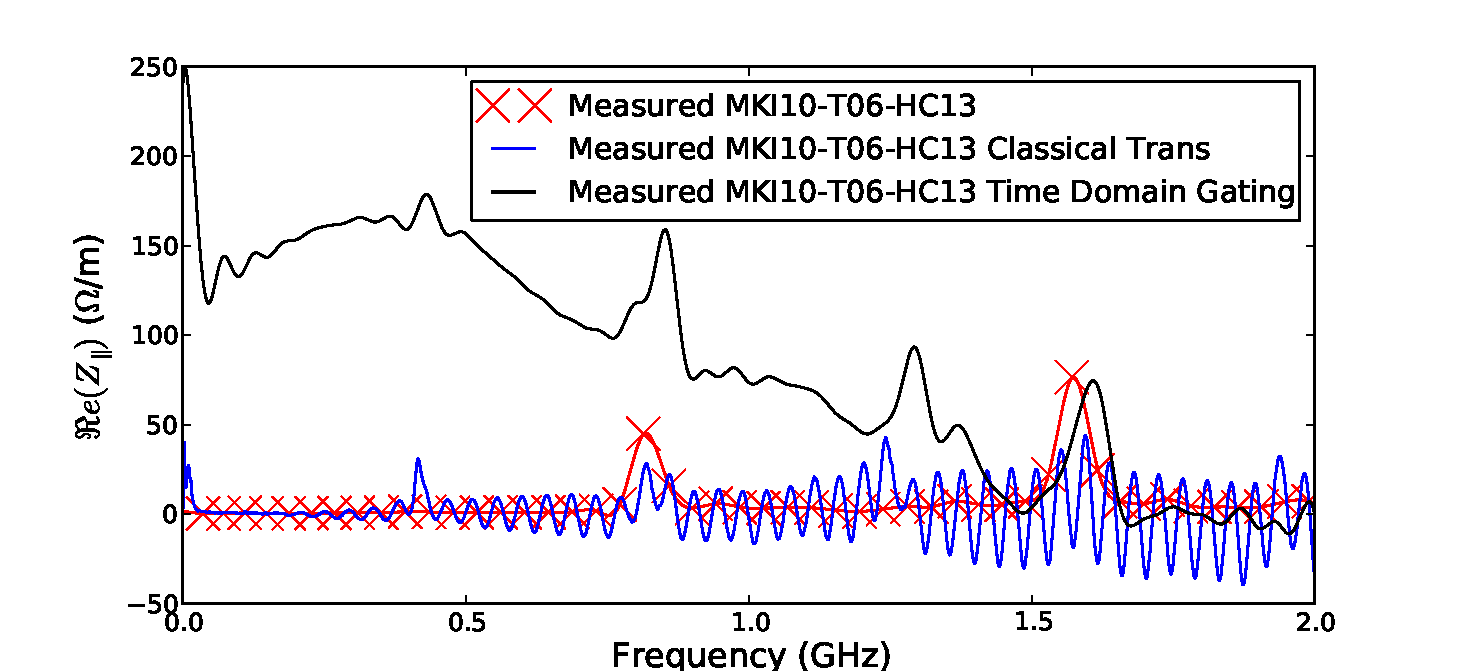
\includegraphics[width=0.5\textwidth]{compMeasurementGating.pdf}
\caption{The beam coupling impedance measurements for a magnet using either time domain gating only, or a matched resistor network in comparison to resonant coaxial wire measurements.}
\label{fig:measComp}
\end{figure}

\section{Power Loss}

To determine the temperatures reached during operation of the MKI under various operational conditions of the LHC it is necessary to calculate the power lost by the beam into the MKIs due to beam-wakefield interactions. Assuming $M$ equi-spaced, equal populated bunches in a circular machine, this is calculated using Eqn.~\ref{eqn:powLoss}, where $f_{0}$ is the revolution frequnecy, $\omega_{0}=2\pi f_{0}$, $e$ is the charge of an electron, $N_{b}$ is the number of particles per bunch, $\lambda(\omega)$ is the beam current spectrum, and $\Re{}e(Z_{\parallel}(\omega))$ is the real component of the longitudinal beam coupling impedance. $\lambda(\omega)$ is highly dependent on the bunch profile, especially the bunch length $t_{b}$. The bunch separation is defined by $\tau_{sep}$

\begin{equation}
P_{loss} = 2 \left( f_{0} e M  N_{b}\right)^{2} \displaystyle\sum\limits_{n = -\infty}^{\infty}  \left| \lambda \left( p M \omega_{0} \right)  \right|^{2} \Re{}e \left[ Z_{\parallel} \left( p M \omega_{0} \right) \right]
\label{eqn:powLoss}
\end{equation}

The power losses are calculated assuming the parameters shown in Tab.~\ref{tab:beamPara}, representing the LHC operational parameters before long shutdown 1, after long shutdown 1 and covering two possible upgrade paths for High-Luminousity LHC using either 50ns or 25ns bunch spacing. The power loss for 15 screen conductors (as most MKIs were prior to LS1) and with the new design with 24 screen conductors (as all MKIs will have post-LS1) is shown in Tab.~\ref{tab:powLoss}. It can be seen that the new beam screen design will see a dramatic reduction in the power lost into the MKIs, from 68W pre-LS1 to between 34-52W after LS1 - a reduction of 20-50\%. However it can be seen that for the proposed HL-LHC parameters the increased beam current will cause the power loss to increase signficantly again - such that the power loss even exceeds the power loss experienced by the MKI8D before TS3 ($\approx 160W$) - indicating that heating may become a problem again if steps aren't taken to remedy the situation.

\begin{table}
\caption{Beam Parameters for different LHC operational modes}
\label{tab:beamPara}
\begin{center}
\begin{tabular}{c | c | c | c | c}
Mode & $\tau_{sep}$ (ns) & $N_{b}$ ($10^{11}$) & $ M $ & $t_{b}$ (ns) \\ \hline 
Pre-LS1 & 50 & 1.6 & $ 1380 $ & 1.2 \\ \hline 
Post-LS1 & 25 & 1.15 & 2808 & 1.0 \\ \hline 
HL-LHC, 50ns & 50 & 3.5 & 1380 & 1.0 \\ \hline 
HL-LHC, 25ns & 25 & 2.2 & 2808 & 1.0 \\ 
\end{tabular}
\end{center}
\end{table}

\begin{table}
\caption{Power Loss for different beam screen arrangements with different beam parameters (see Tab.~\ref{tab:beamPara})}
\label{tab:powLoss}
\begin{center}
\begin{tabular}{c | c | c}
Mode & 24 screen cond. & 15 screen cond. \\ \hline 
Pre-LS1 & 20-35 & 68 \\ \hline 
Post-LS1 & 34-52 & 117 \\ \hline 
HL-LHC, 50ns & 151-240 & 538  \\ \hline 
HL-LHC, 25ns & 125-191 & 432  \\ 
\end{tabular}
\end{center}
\end{table}

\section{Future Plans}

Following from the possibility of recurring heating problems in the MKIs under HL-LHC parameters even with the new beam screen design a number of proposal have been made to reduce the temperature the MKIs might experience. One effort is to increase the rate of power evacuation from the device itself by improving the ability of the magnet to radiate thermal energy and by considering additional cooling solutions \cite{mkiCooling}. In addition it's being considered how to reduce the power loss to the structure further. If the ferrite yoke is well screened (as it is with the new beam screen design) the resonant impedance profile seen in Fig.~\ref{fig:allNewMKIImp} is determined by the overlap between the screen conductors and the external cylinder at the capactively coupled end, such that the resonant frequency $f_{res}$ is given by

\begin{equation}
f_{res} = \frac{n c}{2 \sqrt{\epsilon_{r}}\left( L_{overlap} + \delta_{fringe} \right)}
\end{equation}

where $n$ is an integer, $epsilon_{r}$ the relative permitivitty of the ceramic tube, $L_{overlap}$ the length of overlap between the screen conductors and the external cylinder and $\delta_{fringe}$ the influence of the fringe fields on the perceived length. It can be seen that by reducing the length of the overlap it would be possible to drastically reduce the interaction with the beam current spectrum as the resonances would be pushed to higher frequencies where the current spectrum is lower. A number of simulations have been carried out using CST particle studio \cite{cst-cite} assuming different lengths of overlap to verify that this path of investigation would be fruitful. Preliminary results (shown in Fig.~\ref{fig:overLapSpec}) indicate that the resonances indeed move to higher frequencies, however how these interact with the beam current spectrum in terms of power loss require more investigation.

\begin{figure}
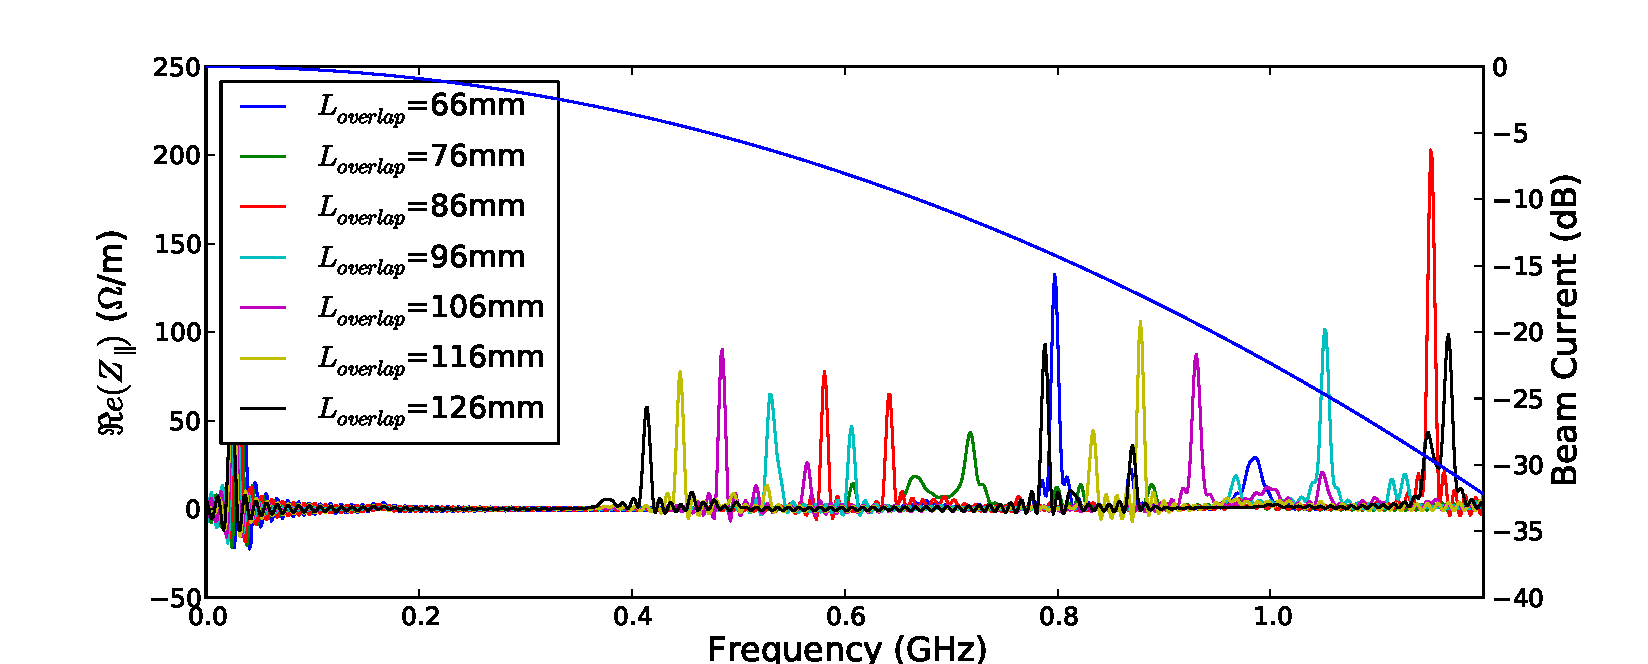
\includegraphics[width=0.5\textwidth]{overlapSpec.pdf}
\caption{The beam current spectrum of a 1ns gaussian bunch compared to the real longitudinal beam coupling impedance for a number of different length overlaps between the screen conductors and the external cylinder.}
\label{fig:overLapSpec}
\end{figure}

\section{Summary}

The upgrades to the beam screen of the LHC injection kickers has been discussed from the view of the beam coupling impedance and beam-induced heating, demonstrating that there will be a substantially lower power loss into the magnets after long shutdown 1 of the LHC is finished. Power loss calculations for HL-LHC indicate that heating of the device may again become a problem and some solutions are discussed with preliminary results shown. In addition some comments on different beam impedance measurement methods are given relating to their use on low beam coupling impedance devices, including benefits and drawbacks in this situation.

%Title format - Title; Authors; Affiliation; conference
%Abstract - Copied from submitted abstract (maybe changed to represent changes in presented paper)
%Introduction
%Body of data
%Conclusion
%Acknowledgements
%References

% Aim of paper - To present the causes of the beam coupling impedance in the beam screen - length of overlap, thickness, screening by conductors. Expected power loss for the new screen design with present and HL-LHC parameters
% Sections:
% Introduction - Brief history of the MKI heating - reference to Mike's paper last year and this year
% Reasons for the impedance - Distinction between well screened and not well screened
% - Increasing number of screen conductors reduces effect of the ferrite
% - Dimensions of the capacitive end changing impedance profile
% - Effect of different ferrites on the 30-40MHz peak if time
% Power loss expectactions for HL-LHC, post LS1 between 15, 19 and New design
%
%
%

% Images to include
% New screen design cross section
% New screen design impedance
% Various lengths of overlap impedance and predicted resonant frequency
% 


\begin{thebibliography}{99}

\bibitem{mkiUpgrade}
M.J. Barnes \emph{et al}., \emph{Upgrade of the LHC Injection Kicker Magnets}, IPAC'13, Shanghai, China, MOPWA030

\bibitem{metral_cham2012}
E. Métral \emph{et al}., \emph{Beam-Induced Heating/Bunch Length/RF and Lessons for 2012}, LHC Performance Workshop, Chamonix 2012, CERN-ATS-2012-069. 

\bibitem{mki-heating}
M.J. Barnes \emph{et al}., \emph{"Analysis of Measured Ferrite Heating of the LHC Injection Kickers and Proposals for Future Reduction of Temperature"}, IPAC'12, New Orleans, USA, 2012, TUPPR090.

\bibitem{mki-heatingTemp}
M.J. Barnes \emph{et al}., \emph{"Beam Induced Ferrite Heating of the LHC Injection Kickers and Proposals for Improved Cooling"}, IPAC'13, Shanghai, China, MOPWA031.

\bibitem{kicker_meas}
H. Day \emph{et al}., \emph{"Evaluation of the Beam Coupling Impedance of new Beam Screen Designs for the LHC Injection Kicker Magnets"}, IPAC'12, New Orleans, USA, 2012, WEPPR071.

\bibitem{mki-ElecBreakdown}
M.J. Barnes \emph{et al}., \emph{"Reduction of Surface Flashover of the Beam Screen of the LHC Injection Kickers"}, IPAC'13, Shanghai, China, MOPWA031.

\bibitem{cst-cite}
\texttt{http://www.cst.com}.

\bibitem{DayThesis}
PhD Thesis, H. Day, 2013.

\bibitem{LHCRF}
P. Baudrenghien \emph{et al}., \emph{"The LHC RF System - Experience with Beam Operation"}, IPAC'11, San Sebastian, 2011, MOPC054.

\bibitem{mkiCoolling}
M. Barnes \emph{et al}., \emph{"Cooling of the LHC Injection Kicker Magnet Ferrite Yoke: Measurements and Future Proposals"}, MOPME075, these proceedings

\end{thebibliography}
\end{document}

